\section{Arkitektur}
Dette kapitlet beskriver krav til konstruksjon eller systemdesign for fellesprosjektet. Konstruksjon av et system skal i prinsippet ikke påvirke de funksjonene som systemet har, men er relatert til de ikke-funksjonelle krav, for eksempel utvidbarhet, vedlikeholdbarhet, ytelse og skalerbarhet. Flerbrukerstøtte er et overordnet ikke-funksjonelt krav, dvs. at mange brukere skal kunne få tilgang til og endre de samme underliggende dataene, fra ulike maskiner på et nettverk.

Ved siden av de spesifiserte ikke-funksjonelle kravene, er det også en del generelle egenskaper ved konstruksjonen som er viktig, for eksempel at funksjoner har definerte grensesnitt i forhold til hverandre og at funksjoner en ønsker å endre på uavhengig av hverandre, ikke er for tett viklet sammen. Det er spesielt to typer koblinger vi er opptatt av å løse opp, nemlig koblinger mellom:

\begin{enumerate}

\item
Applikasjonsdata (modell) og grafisk brukergrensesnitt (GUI)

\item
Applikasjonsdata, slik de representeres mens applikasjonen er i bruk, og deres persistente representasjon på fil eller i en database. 

\end{enumerate}

Den andre av disse er konstruksjonsmessig knyttet til kravet om flerbrukerstøtte, som vi etter hvert skal se i de etterfølgende kapitlene. Kapittel 3.1 beskriver en overordnet systemarkitektur for de som har både SU, DB og KTN. For de som ikke tar DB, KTN og / eller MMI, vil det være noen endringer som er beskrevet i Kapittel 3.5.

\subsection{Trelags applikasjonsarkitektur}

Det er vanlig å dele applikasjoner i tre deler, med hver sin funksjon (se Figur 2):

\begin{enumerate}

\item
Brukergrensesnittet, i vårt tilfelle et GUI, er den delen som brukeren interagerer direkte med gjennom bl.a. skjerm, mus og tastatur. GUI gir brukeren mulighet for å navigere i og se på data og gir tilgang til funksjoner for å endre dataene. Strukturen på GUI er nært knyttet til strukturen til de dataene, slik den er beskrevet i f.eks. et UML klassediagram, men først og fremst basert på hva brukeren ønsker å gjøre. Implementasjonen av GUI gjøres ofte ved hjelp av et GUI-rammeverk og som regel i samme programmeringsspråk som applikasjonen forøvrig, i vårt tilfelle Java og Swing.

\item
Modellen er alle objektene i den kjørende applikasjonen som brukeren er interessert i å få tilgang til. Disse objektene eksisterer uavhengig av om GUI viser dem, og det er ikke umulig eller unaturlig å ha flere typer brukergrensesnitt som gir tilgang til de samme applikasjonsdataene, eller kun deler av disse. Modellen inneholder både data og regler for hvordan disse kan manipuleres, og sistnevnte kalles ofte applikasjonslogikk. Modellen vil typisk være beskrevet ved hjelp av UML klassediagram, som et ledd i analysearbeidet i forbindelse med. kravspesifikasjonen. Dersom en bruker et objektorientert språk som Java, vil både data og logikk implementeres vha. klasser. 

\item
Persistensdelen håndterer lagring av modellen mellom hver kjøring av applikasjonen, og er typisk støttet av en database eller et filsystem. Igjen er det ikke umulig eller unaturlig å tenke seg at de samme dataene kan lagres på ulike vis av en og samme applikasjon, f.eks. som en XML-fil, i en XML-database eller i en relasjonsdatabase. Førstnevnte passer bra for dokumentorienterte enbrukerapplikasjoner, sistnevnte passer bra for flerbrukerapplikasjoner med mer komplekse data og spørringer, og hvor det kan være behov for transaksjonshåndtering. Beskrivelsen av de persistente dataene er avhengig av den underliggende mekanismen, og kan være XML-dtd og –skjema og ER-diagram og SQL-skript.

\end{enumerate}

Ved konstruksjon er det viktig å tenke på både den interne strukturen i hver av de tre delene, som gjerne følger bestemte regler eller mønster for konstruksjon, og grensesnittet og samspillet mellom dem. Den interne strukturen i brukergrensesnittet og forholdet mellom brukergrensesnittet og modellen er en sentral del av MMI-faget. DB-faget tar for seg forholdet mellom applikasjonen og databasebasert persistens og struktur og egenskaper for databasen. Dersom disse tre delene av applikasjonen er skilt fra hverandre med et nettverk, har KTN-faget sitt å si om hvordan dette bør håndteres. SU-faget har den modellen/applikasjonslogikken og den overordnede strukturen eller arkitekturen, som sitt anliggende.

\subsection{Fra enbrukerapplikasjon til klient-tjener-arkitektur}

Applikasjonsarkitekturen som er beskrevet over, er et greit utgangspunkt for å konstruere en enbrukerapplikasjon. I dette prosjektet kan en forestille seg at en i første omgang støtter filbasert lagring med XML som format, som illustrert i Figur 3.

I en dokumentorientert applikasjon vil hele modellen bli lagret som en transaksjon, og grensesnittet mellom modellen, dvs. de to pilene, vil være nokså enkelt. Den venstre pilen representerer funksjonen modell-til-XML-oversetting, mens den høyre pilen tilsvarer den motsatte funksjonen XML-til-modell-oversetting. Merk at funksjonene håndterer kun hele modeller, så det er ikke behov for å oversette delmodeller i den ene eller andre retning. Det kan selvsagt være lurt å bryte funksjonene ned i mindre deler, basert på modellens struktur, men dette er konstruksjonsdetaljer som ikke påvirker grensesnittet representert ved pilene.

En ulempe med denne applikasjonsarkitekturen er at XML-filer ikke kan leses eller skrives over nettverket (med mindre en utnytter nettverkstøtten i filsystemet), f.eks. http- eller ftp-URL’er. Det skal imidlertid ikke så mye endring til for å håndtere dette, som vist i Figur 4.

Her vil klientapplikasjonen være så godt som uendret. Den eneste forskjellen er at lesing og skriving av XML-dokumentet skjer over nettverket, ved hjelp av en eller annen protokoll. Dersom en bruker URL-er til å adressere tjeneren og Java sin innebygde støtte for lesing og skriving til URL-oppkoblinger, så er det lite omkoding som trengs. I tillegg er det et stort poeng at endringen er intern i persistensdelen, så GUI og modellen er ikke berørt, kanskje bortsett fra dialogelementer for visning og innskriving av URL-en.
Tjeneren vil i dette tilfellet være nokså enkel, da den kun skal kunne ta i mot en oppkobling og kunne lese fra og skrive til nettverket og henholdsvis skrive til og lese fra fil.

Dersom en deler opp persistensdelen i en del som håndterer oversettingen til og fra XML og en del som håndterer lesing og skriving, er det relativt enkelt å få til en kombinasjon av disse to. Dette er vist i Figur 5.

Dette krever at overgangen mellom XML-oversettingen og lesing/skriving av XML-dokumentet er tydelig, f.eks. definert i et eget Java-grensesnitt og at en har klasser for filbasert og nettverksbasert I/O som implementerer dette grensesnittet. Dette tilsvarer forøvrig arkitekturen til først inkrement, med HTTP som nettverksprotokoll.

Selv om vi i de to siste figurene har innført en tjener, er tjeneren såpass enkel at arkitekturen ikke håndterer at flere brukere får tilgang til de samme dataene. Rollen til tjeneren er foreløpig kun knyttet til lagring og ikke til delt tilgang for flere klienter til felles data. For å få det til er det vesentlig at tjeneren også har et modell-lag og mekanismer for å håndtere delt tilgang. Figur 6 skisserer en arkitektur for å håndtere dette, men figuren forteller bare en del av historien.

Merk at modellene kan godt være implementert av akkurat de samme klassene og vi kan godt bruke XML som overføringsformat. I tillegg til å innføre et modell-lag i tjeneren, er det viktig å definere regler for samspillet mellom tjenerens modell og modellen i hver klient:

\begin{enumerate}

\item
Tjenerens modell er den offisielle modellen.

\item
Klientene må ved hver vesentlige endring lokalt, overføre endringen til tjeneren, for å unngå inkonsistens mellom lokal og offisiell modell.

\item
Tjeneren må, når den mottar endringer fra en klient, integrere endringene i sin modell, og videreformidle endringene til de andre klientene.

\item
Klientene må være beredt til å motta endringer fra tjeneren og integrere disse i sin egen lokale modell.

\end{enumerate}

Kommunikasjonen mellom tjeneren og klientene har altså som formål å sikre konsistens mellom lokale modeller og den tjenerens offisielle, og dataene som sendes over nettverket må være tilpasset dette formålet, for eksempel:

\begin{enumerate}

\item
Både tjeneren og klientene må kunne overføre fragmenter av modellen og ikke bare hele modellen som i enbrukerapplikasjonen

\item
Overføringen må inneholde informasjon om hva slags endring som skal gjøres i den andre enden, f.eks. slette, oppdatere eller opprette objekter

\item
En må kunne angi hvilke deler av den offisielle modellen som skal endres, f.eks. hvilket attributt som skal endre, hvilket objekt som skal slettes eller hvilken relasjon som skal opprettes

\end{enumerate}

Det som overføres i begge retninger mellom klient og tjener kan sees på som en kommando med tilhørende data, og en viktig del av designarbeidet er å definere kommandoene slik at dekker behovene over og bestemme hvordan de skal kodes i XML og formidles over HTTP.

Som vi ser er persistenslaget omdøpt til kommunikasjon i figuren over, men det betyr ikke at persistens er mindre viktig. Vi må fortsatt sikre at dataene overlever når applikasjonen avslutter, så persistensmekanismen må gjeninnføres, slik vi har vist i Figur 7.

For å sikre at modellen kan gjenopprettes hvis tjeneren krasjer, er det viktig at databasen blir oppdatert i takt med tjenerens modell. Hvilken som oppdateres først, modellen eller databasen, er en smakssak, men begge bør gjøres før klientene oppdateres, for å minimere muligheten for at krasj underveis. Det overordnede poenget er at det er databaseinnholdet som er grunnlaget for å gjenopprette modellen ved krasj eller vedlikehold av tjeneren. Derfor er databasen til syvende og sist mer ”offisiell” enn modellen i den kjørende tjeneren, siden det er den vi sitter igjen med når strømmen slås av.

\subsection{Arkitektur og Java-programmering}

Overgangen fra abstrakte arkitekturfigurer som vist over, til praktisk Java-koding kan kanskje virke vanskelig. Dette får dere mer informasjon om på (øvings?)forelesningene, men her er to vesentlige tips å ta med seg:

\begin{enumerate}

\item
Arkitekturen er en funksjonell nedbrytning av applikasjonen, og denne nedbrytningen kan være grei å bruke når en skal definere Java-pakkestrukturen for prosjektet. F.eks. kan en ha en A-pakke på toppen med pakker for GUI, modell og persistens under. Alle GUI-klasser vil ha A.gui som pakkeprefiks, for eksempel A.gui.ProduktPanel, mens modellklassene vil ha A.modell som pakkeprefiks, for eksempel A.modell.Produkt.

\item
Definer koblingen mellom lagene i arkitekturen ved hjelp av Java-interface, for eksempel A.persistens.ModellLeser og A.persistens.ModellSkriver for lesing og skriving av modellen. Implementasjonen av disse grensesnittene kan godt ligge i egne underpakker, f.eks. A.persistens.fil.Model.ModellLeserImpl og A.persistens.fil. ModellSkriverImpl.

\end{enumerate}

\subsection{Databaselagring}

Data skal lagres i en relasjonsdatabase, som tjeneren kommuniserer med ved hjelp av JDBC. Alle endringer som skjer i systemet, f. eks. at  en ny avtale legges inn, skal føre til at databasen oppdateres for å reflektere den nye situasjonen. Tjeneren skal kunne krasje eller skrus av, og deretter skrus på igjen, uten at data går tapt. Tjeneren skal lese inn data fra databasen når den starter opp.

Data som tjeneren tar imot fra klienten er strukturert som XML. Denne skal derfor analyseres av tjeneren, og informasjonen i den legges inn i databasen på en hensiktsmessig måte. En del av prosjektoppgaven er å utforme en hensiktsmessig datamodell, implementere denne i en SQL-database, og lage et program som fyller den med data på grunnlag av XML-filen. 

Tjeneren og databasen skal kommunisere ved hjelp av JDBC, som er standardbiblioteket for databasekommunikasjon i Java. JDBC vil bli forelest i TDT4145 Datamodellering og databasesystemer.

All informasjon som tjeneren sender til klientene/gateway skal være korrekt i henhold til databasen. En mulig måte å gjøre dette på, er å utføre spørringer mot databasen hver gang. Å cache deler av data i tjeneren kan være mer effektivt, men kan også øke kompleksiteten. Dere står imidlertid fritt til å implementere dette slik dere finner det for godt.

\subsection{Endringer i krav for grupper som ikke har alle fagene}

\begin{enumerate}

\item
For de som ikke har DB skal all persistens bli ivaretatt av filsystemet. 

\item
De som ikke har MMI må selv lage et enkelt brukergrensesnitt for å kunne teste systemet. Dette brukergrensesnittet kan gjerne være kommandobasert. 

\item
Alle krav i kravlista relatert til nettverk utgår for de som ikke har KTN. 

\end{enumerate}

\subsection{Eksempelkode for et personregister – ”kjerneapplikasjonen”}

Eksempelkoden er en enkel adressebok der brukeren kan legge til, fjerne og redigere en liste med personer og tilhørende personalia som fødselsdag og e-postadresse. Vi har tradisjonstro valgt å kalle denne for ”kjerneapplikasjonen”, men er hovedsakelig ment som en resurs hvor gruppene kan plukke kodesnutter og/eller se eksempler på hvordan ting kan implementeres. Noe av tanken bak dette er også å gi dere trening i å sette dere inn i andres/eksisterende kode.

\subsubsection{Installasjon}

Eksempelkoden/kjerneapplikasjonen er gjort tilgjengelig som ei zip-fil på Web/it’s learning. Gjør følgende for å få tilgang til kildekoden fra zip-fila i Eclipse:

\begin{enumerate}

\item
Pakk ut fila kjerne.zip (dobbeltklikk på fila i Utforsker) i en midlertidig katalog (f.eks. m:\textbackslash tmp\textbackslash ).  Denne midlertidige katalogen kan ikke være den samme som du velger som Workspace i steg 2. Fila oppretter en ny katalog, kjerne, i den valgte katalogen (f.eks. m:\textbackslash tmp\textbackslash kjerne\textbackslash )

\item
Start Eclipse. I Workspace Launcher som kommer opp ved oppstart velger du Workspace-katalogen der du har kildekoden din (f.eks. m:\textbackslash eclipse).  Opprett en katalog om du ikke allerede har en katalog til kildekoden din.

\item
Opprett et Eclipse-prosjekt for kjerneapplikasjonen
\begin{enumerate}

\item
I Eclipse, opprett et nytt prosjekt for kjerneapplikasjonen ved å velge File - New - Project.  Dialogboksen New Project kommer opp.

\item
I dialogboksen New Project velger du Java Project og klikker Next>.

\item
Kall prosjektet ”kjerne” (føres i innskrivingsboksen Project name) i neste skjermbilde, og klikk Finish.

\end{enumerate}

\item
Importer kildekoden til kjerneapplikasjonen inn i Eclipse-prosjektet

\begin{enumerate}

\item
Importer kjerneapplikasjonen ved å velge File -> Import.  Dialogboksen Import kommer opp.

\item
I dialogboksen velg 'File system' under Select an import source:, og klikk Next

\item
I innskrivingsboksen From directory skriver du enten inn stien der du pakka ut kjerne.zip (f.eks. m:\textbackslash tmp\textbackslash kjerne\textbackslash ) eller bruker Browse-knappen for å finne katalogen.

\item
Klikk på knappen Select all og så Finish.

\item
Svar Yes to all på eventuelle spørsmål som dukker opp under importeringa av kildekoden.

\end{enumerate}

\end{enumerate}

Du har nå tilgang til kildekoden i Eclipse.

\subsubsection{Arkitektur}

Kjerneapplikasjonen bygger på en trelagsarkitektur. Det vil si at applikasjonen er delt inn i tre lag: et lag for brukergrensesnitt, et lag for datamodell og et lag som tar vare på persisterings.

\begin{figure}[H]
    \centering
    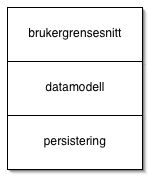
\includegraphics{resources/layering-application.jpg}
    \caption{Application layering}
    \label{fig:layering-application}
\end{figure}

Hvert av lagene i applikasjonen tar seg av ulike funksjoner. Alle Java-klassene som implementerer brukergrensesnittet og funksjonaliteten forbundet med brukergrensesnittet, hører hjemme i brukergrensesnittlaget. Klassene som implementerer datastrukturene i kjerneapplikasjonen og tilhørende funksjonalitet, hører hjemme i datamodell-laget. I persistersistens-laget ligger klassene som tar seg av å lagre og lese inn data fra disk. I praktisk Java har vi delt koden for kjerneapplikasjonen inn i Java-pakker. En Java-pakke for hvert av lagene i applikasjonen:

\begin{figure}[H]
    \centering
    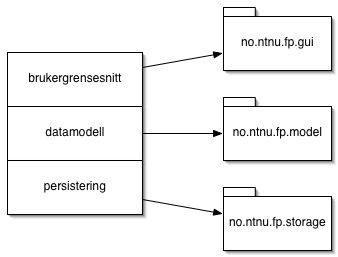
\includegraphics[width=\textwidth]{resources/layering-corresponding-java-packets.jpg}
    \caption{Layering with corresponding java packages}
    \label{fig:layering-corresponding-java-packets}
\end{figure}

Hensikten med trelagsarkitekturen er å redusere koblinga mellom delene av applikasjonen. Det er derfor slik at hvert lag kun kommuniserer med laget over og/eller under. For eksempel: brukergrensesnittlaget kan kommunisere med datamodell-laget og datamodell-laget kan kommunisere med persisteringslaget, men brukergrensesnittlaget kan ikke kommunisere direkte med persisteringslaget og omvendt.

\subsubsection{Design}

\begin{figure}[H]
    \centering
    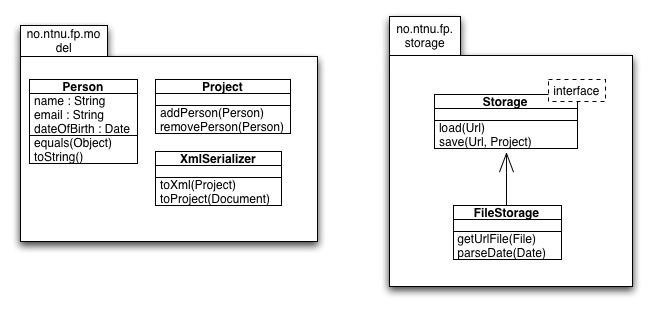
\includegraphics[width=\textwidth]{resources/design-classdiagram.jpg}
    \caption{Class diagram}
    \label{fig:classdiagram}
\end{figure}

\subsubsection{Datamodell-laget}

Datamodell-laget består av fire klasser: Person, Project og XmlSerializer.  Disse klassene befinner seg i Java-pakken: no.ntnu.fp.model.

Person- og Project-klassene er dataklassene i kjerneapplikasjonen. Personklassen er en datastruktur som holder informasjonen om personene i adresseboka. Project-klassen er en samling av en eller flere Personobjekter.

XmlSerializer-klassen konverterer data mellom XML-tekst og Java-objekter. Gitt en XML-tekst, konverterer denne klassen til enten Person- eller Gruppeobjekter avhengig av hvilken metode som kalles. Gitt Person- eller Project-klasse konverterer XmlSerializer til XML-tekst. 

\subsubsection{Persisteringslaget}

Persisteringslaget består av et Java-interface, Storage, og en klasse som implementerer dette Java-interfacet, FileStorage. Klassene og interfacet befinner seg i Java-pakken: no.ntnu.fp.storage.

FileStorage-klassen implementerer fellesfunksjonalitet som kreves for å lagre objekter fra datamodell-laget til fil, både til XML-filer og kommaseparert format.

\subsubsection{Programsekvenser}

Under beskrives de viktigste sekvensene i kjerneapplikasjonen. For leselighetens skyld, er objektene i sekvensflyten gitt det samme navnet som klassen, prefikset av en a eller an. For eksempel: et objekt av klassen Group omtales i sekvensdiagrammet som aGroup, og et objekt av Storage-klassen omtales i sekvensdiagrammet som aStorage.


\subsubsection{Programsekvens: Åpne fil}

Følgende programsekvens eksekveres når brukeren velger File - Open:

\begin{figure}[H]
    \centering
    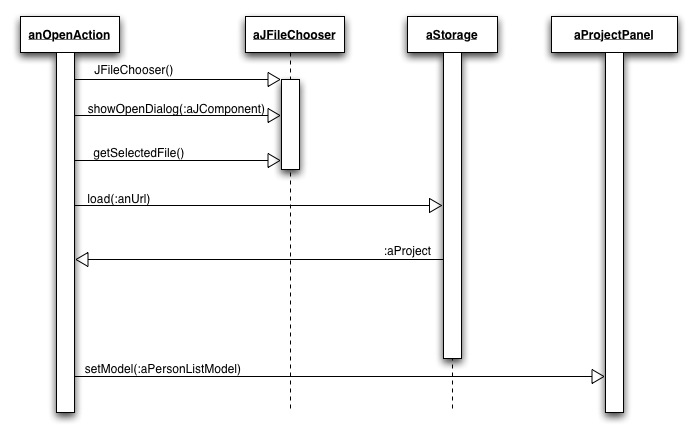
\includegraphics[width=\textwidth]{resources/sequence-open-file.jpg}
    \caption{Sequence diagram for opening a file}
    \label{fig:sequence-open-file}
\end{figure}

\subsubsection{Programsekvens: Lagre til fil}

Følgende programsekvens eksekveres når brukeren velger File - Save:

\begin{figure}[H]
    \centering
    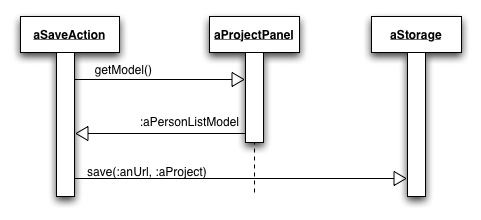
\includegraphics[width=\textwidth]{resources/sequence-save-file.jpg}
    \caption{Sequence diagram for saving a file}
    \label{fig:sequence-save-file}
\end{figure}

\subsubsection{Nettverk}

Dette kapittelet er ment som en hjelp for å komme i gang med å implementere nettverksstøtte for kjerneapplikasjonen. Kjerneapplikasjonen er tilrettelagt for nettverkskommunikasjon mellom to applikasjoner på hver sin datamaskin. Når du starter kjerneapplikasjonen vil du se et innslag på menylinja som heter Net. Om du trekker ned denne menyen har du tre valg: Connect, Disconnect, Accept incoming... Disse tre funksjonene har følgende funksjonalitet:

\begin{enumerate}

\item
Med Accept incoming... venter applikasjonen på innkommende nettverkskoblinger fra en applikasjon på en annen datamaskin.

\item
Connect kobler applikasjonen opp til en applikasjon som a) kjører på en annen datamaskin, og b) venter på innkommende nettverksoppkoblinger (dvs. brukeren har valgt Net - Accept incoming...). 

\item
Disconnect bryter oppkobling mot en annen kjerneapplikasjon.

\end{enumerate}

PS: I koden dere har fått utlevert er ingen av disse tre funksjonene implementerte. Om man prøver å kjøre de, får man bare opp en dialogboks som sier Function not implemented. Det er fordi oppgaven til nettverksfaget er akkurat det å implementere denne funksjonaliteten.

Koden for kjerneapplikasjonen kommer med en pakke som heter no.ntnu.fp.net. Denne pakken inneholder to Java-interfacer, Connection og MessageListener, samt en Java-klasse, ConnectionWorker.

Connection skal implementeres med koden som trengs for å a) koble opp mot en annen maskin, b) vente på oppkoblinger fra en annen maskin, c) motta meldinger fra en annen maskin, og c) sende meldinger til en annen maskin. Dataprotokollen som brukes er det samme XML-formatet som brukes for lagring.  

Sekvensen i Figur \ref{fig:sequence-core-application-receive-data} viser hva som skjer når en kjerneapplikasjon mottar data over nettverket. Merk: dette er kun prinsippene, koden må dere selv implementere. I tillegg til at dere må implementere Connection-interface'et ser dere fra sekvensen over at dere også må implementere MessageListener-interface'et slik at XML-strengen som mottas fra netter blir konvertert til et Personobjekt som kan legges til i et Project-objekt.

\begin{figure}[H]
    \centering
    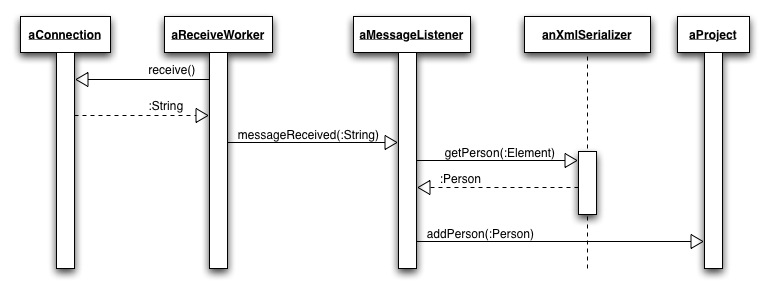
\includegraphics[width=\textwidth]{resources/sequence-core-application-receive-data.jpg}
    \caption{Core application receives data over the network}
    \label{fig:sequence-core-application-receive-data}
\end{figure}

Hva så med å sende data? Sekvensen i Figur \ref{fig:sequence-property-change-listener} viser hva dere må implementere for å få det til. Dere må implementere en PropertyChangeListener som lytter på endringer i Group-objektet. Denne PropertyChangeListener-klassen konverterer Personobjektet som er endret/lagt til over til XML ved hjelp av no.ntnu.fp.model.XmlSerializer-klassen. XML-en sendes med send-metoden i Connection-klassen.

\begin{figure}[H]
    \centering
    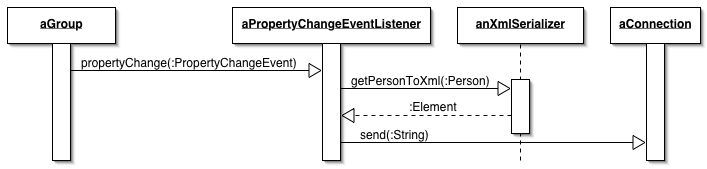
\includegraphics[width=\textwidth]{resources/sequence-property-change-listener.jpg}
    \caption{PropertyChangeListener}
    \label{fig:sequence-property-change-listener}
\end{figure}

Sekvensen i Figur \ref{fig:sequence-connect-to-core-application} viser stegene for å koble seg opp mot en annen kjerneapplikasjon. Igjen: koden må dere selv skrive. Her bruker vi også ConnectAction-klassen. Denne ligger i no.ntnu.fp.gui-pakken, og inneholder i dag bare testkode for å åpne en dialogboks som forteller deg at funksjonen ikke er implementert. Dere må selv implementere koden i ConnectAction-klassen slik at den kaller de riktige objektene og sette opp applikasjonen slik at den kan sende og motta data fra/til applikasjonen den kobler seg til.

\begin{figure}[H]
    \centering
    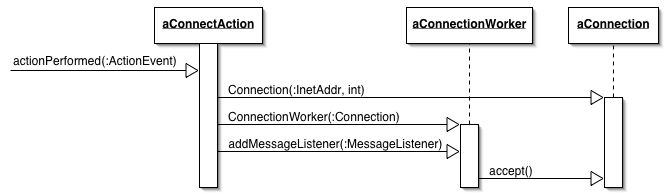
\includegraphics[width=\textwidth]{resources/sequence-connect-to-core-application.jpg}
    \caption{Connecting to another core application}
    \label{fig:sequence-connect-to-core-application}
\end{figure}

Hver av de tre menyinnslagene Connect, Disconnect og Accept incoming har korresponderende action-klasser i no.ntnu.fp.gui-pakken: ConnectAction, DisconnectAction og AcceptAction. Som med ConnectAction-klassen, må dere selv implementere den riktige funksjonaliteten i de to andre action-klassene.
